\section{Технологическая часть}

В данном разделе будет представленно обоснование выбора языка и среды программирования, ...

\subsection{Выбор средств программной реализации}
В качестве языка программирования был выбран Python 3, ввиду следующих факторов.

\begin{itemize}
	\item За время обучения был накоплен существенный опыт в использовании данного средства, что позволит сократить время разработки программы.
	\item Язык поддерживает объектно-ориентированный подход, что полезно при структурировании большого количества схожих объектов, которые были выделены ранее.
	\item Наличие библиотек для создания графического интерфейса, визуализации графов и временных диаграмм, которые необходимы для более наглядной демонстрации работы программы.
\end{itemize}
\qquad
В качестве среды разработки был выбран PyCharm по следующим причинам.
\begin{itemize}
	\item Данная IDE предоставляется бесплатно для пользования в учебном заведении\cite{tech:pycharm}.
	\item Имеется значительный опыт в использовании данной среды разработки.
	\item Представлен удобный набор инструментов для написания, тестирования и отладки кода.
\end{itemize}

\subsection{Используемые библиотеки}
На выбранном языке Python написаны библиотеки, позволяющие упростить визуализацию данных. Перечислим те, которые были использованы при разработке программы.

При разработке графического интерфейса пользователя использовался
PyQt5. Qt является популярным кроссплатформенным графическим фреймворком\cite{libs:pyqt}. Наличие среды для разработки интерфейсов Qt Designer значительно упрощает работу с данной библиотекой при создании GUI.

При создании графов применялась библиотека networkx. Она позволяет генерировать различные типы случайных графов, что может быть использовано при тестировании и исследовании реализованной программы для создания случайных транспортных систем. Также имеется возможность привязки необходимой информации непосредственно к узлам и рёбрам графов.

Для визуализации временной диаграммы маршрутов и графа транспортной системы использовалась библиотека plotly\cite{libs:plotly}.

\subsection{Интерфейс программы}
Для удобства задания и изменения параметров системы был разработан графический интерфейс, представленный на рисунках \ref{gui:main} -- \ref{gui:warehouse}.

В главном окне программы происходит отображение имеющихся пунктов транспортной системы, а также её схематичной визуализации в виде графа. В данном окне пользователь может совершить следующие действия.

\begin{figure}[hp]
	\begin{center}
		{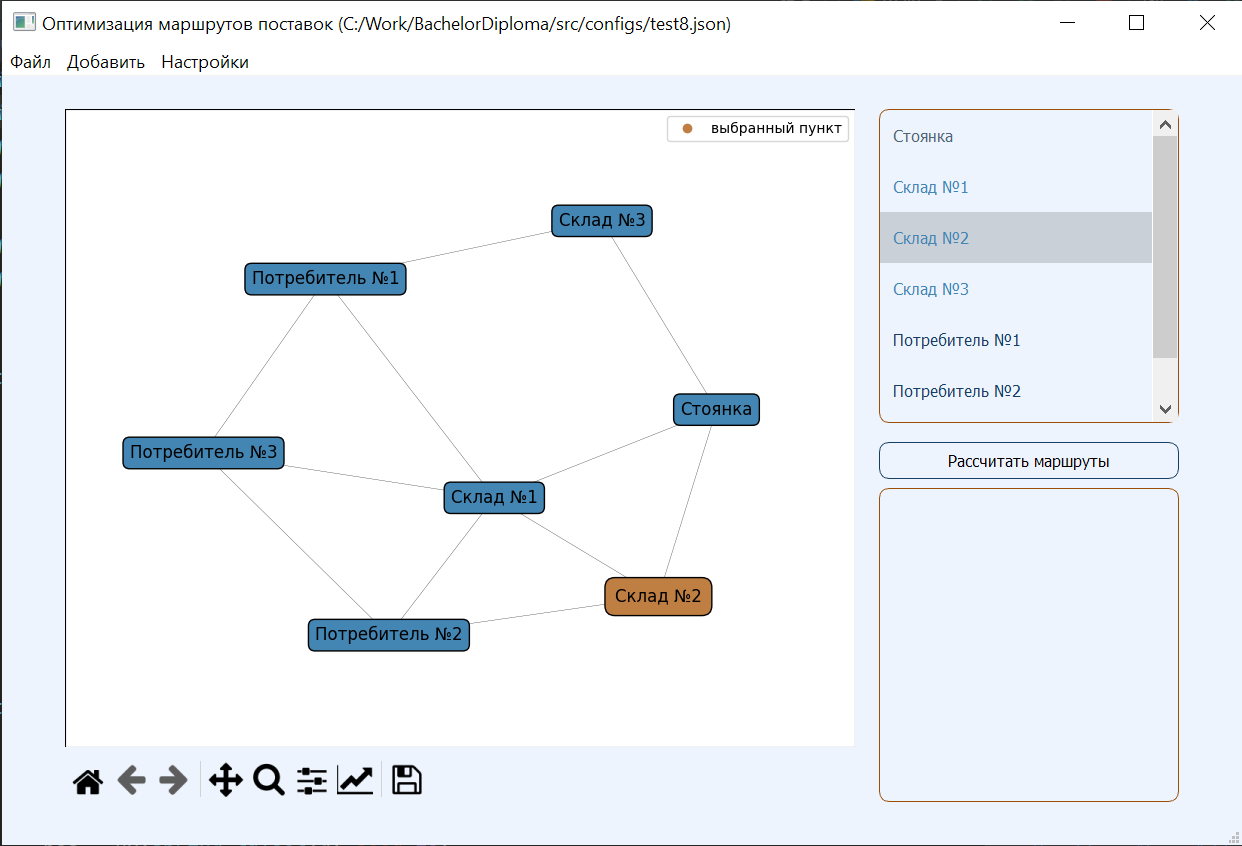
\includegraphics[scale=0.75, angle=0, page=1]{img/main_page.png}}
		\caption{Интерфейс главного окна программы}
		\label{gui:main}
	\end{center}
\end{figure}

\begin{itemize}
	\item Перейти к окну редактирования параметров пункта.
	\item Добавить новый пункт в систему.
	\item Импортировать транспортную систему из указанного файла.
	\item Экспортировать текущее состояние системы в файл.
	\item Настроить прочие параметры системы.
	\item Вызвать построение плана маршрутов.
	\item Посмотреть график маршрутов на временной диаграмме.
\end{itemize}

\qquad
На рисунке \ref{gui:parking} изображено окно изменения параметров стоянки. В данном окне пользователь может совершить следующие действия.

\begin{figure}[hp]
	\begin{center}
		{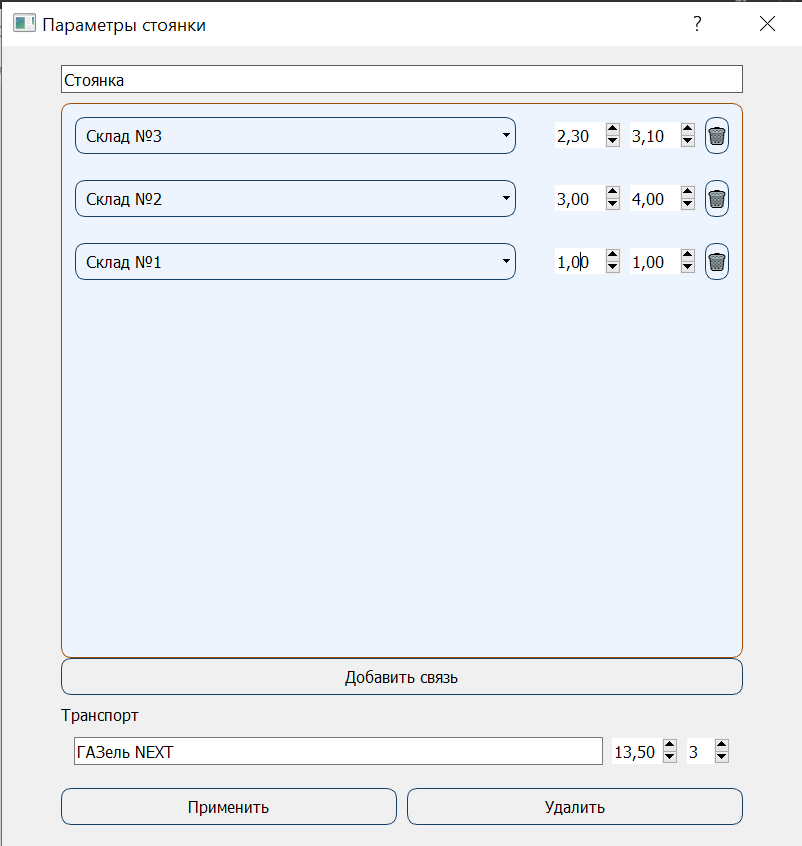
\includegraphics[scale=0.8, angle=0, page=1]{img/parking_page.png}}
		\caption{Интерфейс окна параметров стоянки}
		\label{gui:parking}
	\end{center}
\end{figure}

\begin{itemize}
	\item Изменить название пункта.
	\item Редактировать существующие дороги до других пунктов, удалять и добавлять новые.
	\item Изменить название, вместительность и количество машин в автопарке.
	\item Применить изменения.
	\item Удалить сущность из системы.
\end{itemize}

Похожий интерфейс имеет окно изменения параметров склада и потребителя, изображённое на рисунке \ref{gui:warehouse}. Оно позволяет дополнительно управлять набором продуктов, составляющих заказ или запас в пункте.

\begin{figure}[hp]
	\begin{center}
		{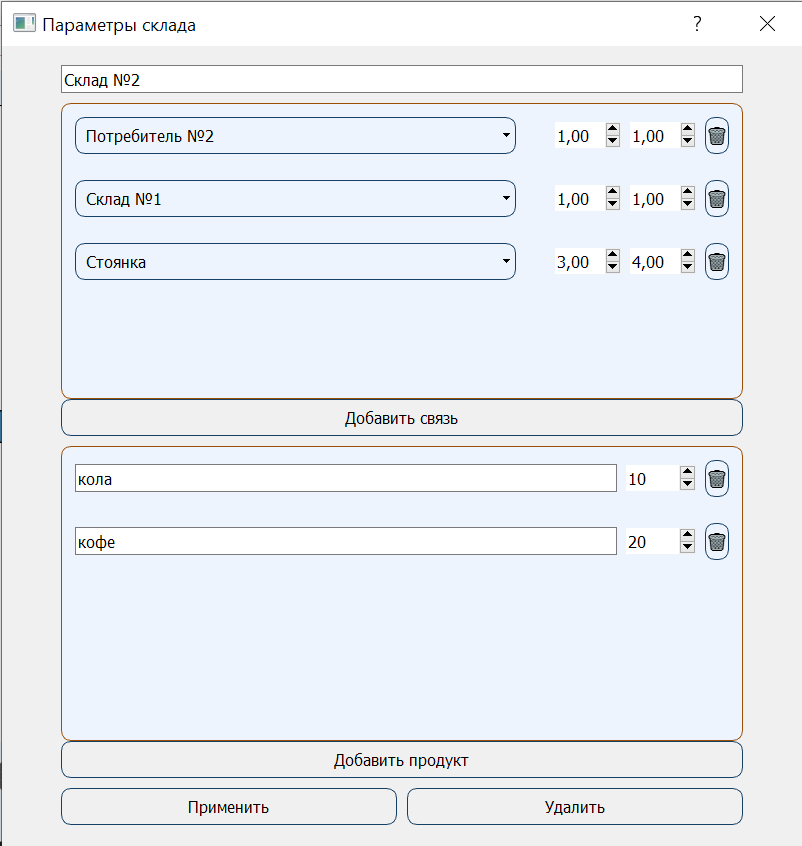
\includegraphics[scale=0.8, angle=0, page=1]{img/warehouse_page.png}}
		\caption{Интерфейс окна параметров склада}
		\label{gui:warehouse}
	\end{center}
\end{figure}


\subsection{Результаты работы программы}
Графический интерфейс также визуализирует результаты составления и оптимизации плана грузоперевозок, что отражают рисунки \ref{demo:routes1} -- \ref{demo:schedule2}. На них изображены результаты работы метода на сети малого и большого размеров. Приведены визуализации и отчёты маршрутов, временная шкала графика передвижения транспорта по узлам сети.

\begin{figure}[h]
	\begin{center}
		{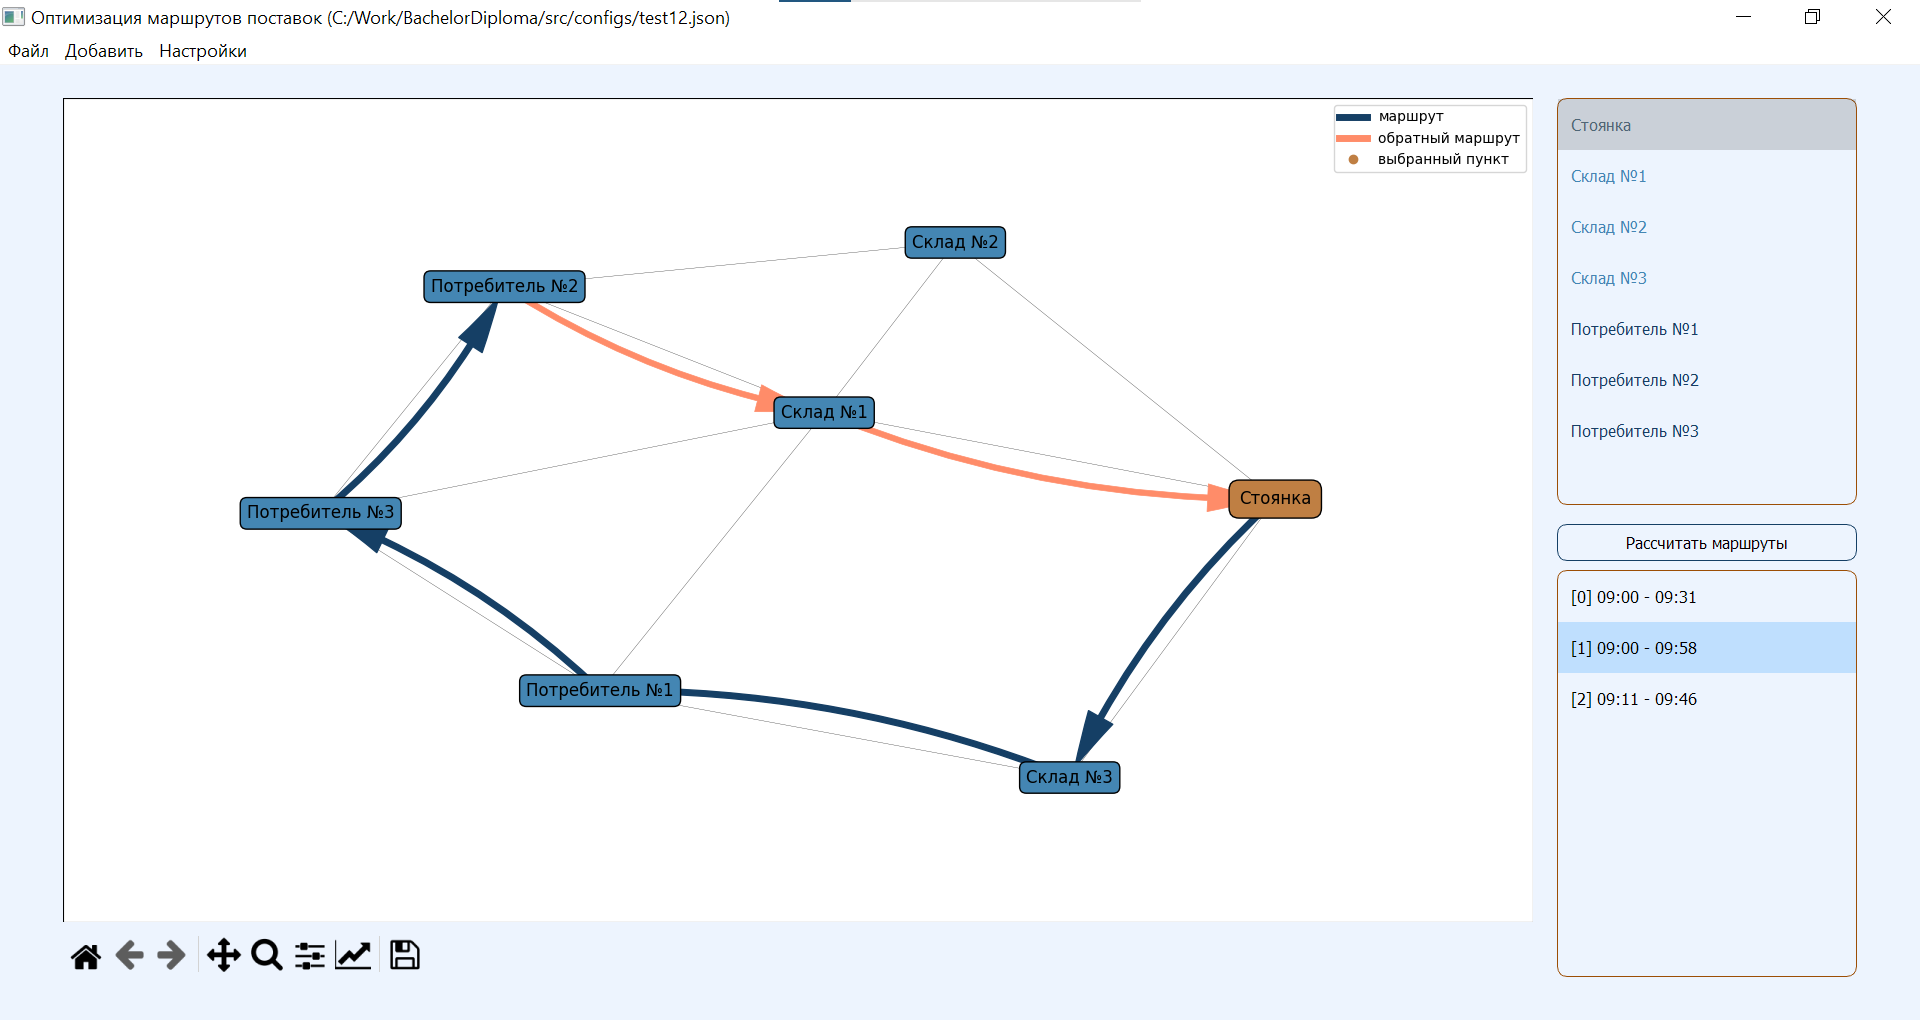
\includegraphics[scale=0.45, angle=0, page=1]{img/demo_routes_1.png}}
		\caption{Пример 1. Визуализация маршрута}
		\label{demo:routes1}
	\end{center}
\end{figure}

\begin{figure}[h!]
	\begin{center}
		{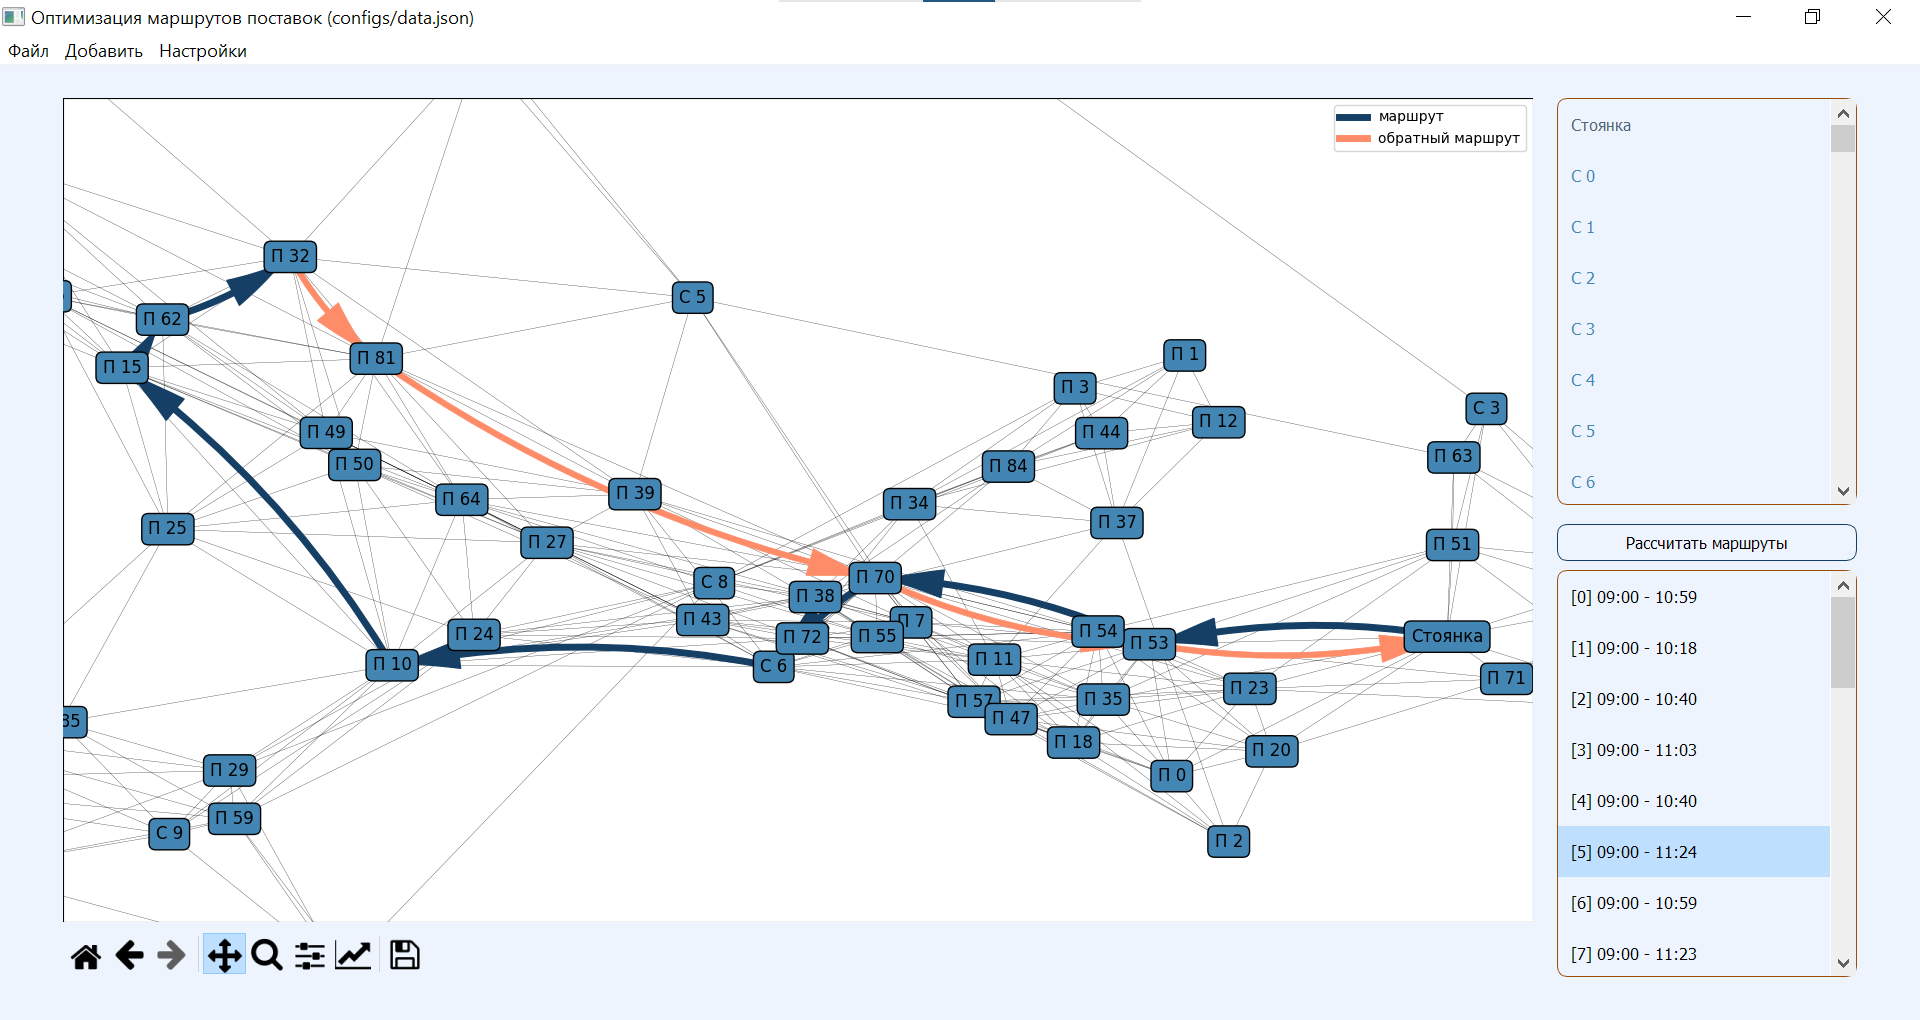
\includegraphics[scale=0.45, angle=0, page=1]{img/demo_routes_2.png}}
		\caption{Пример 2. Визуализация маршрута}
		\label{demo:routes2}
	\end{center}
\end{figure}

\begin{figure}[h!]
	\begin{center}
		{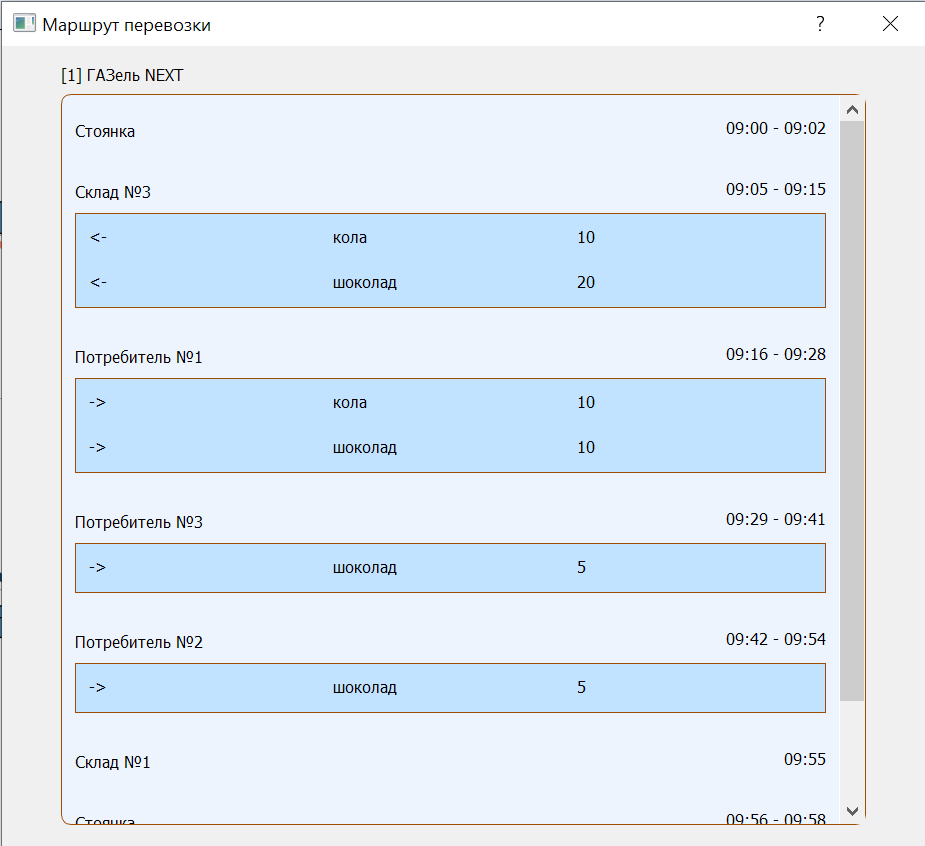
\includegraphics[scale=0.6, angle=0, page=1]{img/demo_route_1.png}}
		\caption{Пример 1. План маршрута}
		\label{demo:route1}
	\end{center}
\end{figure}

\begin{figure}[h!]
	\begin{center}
		{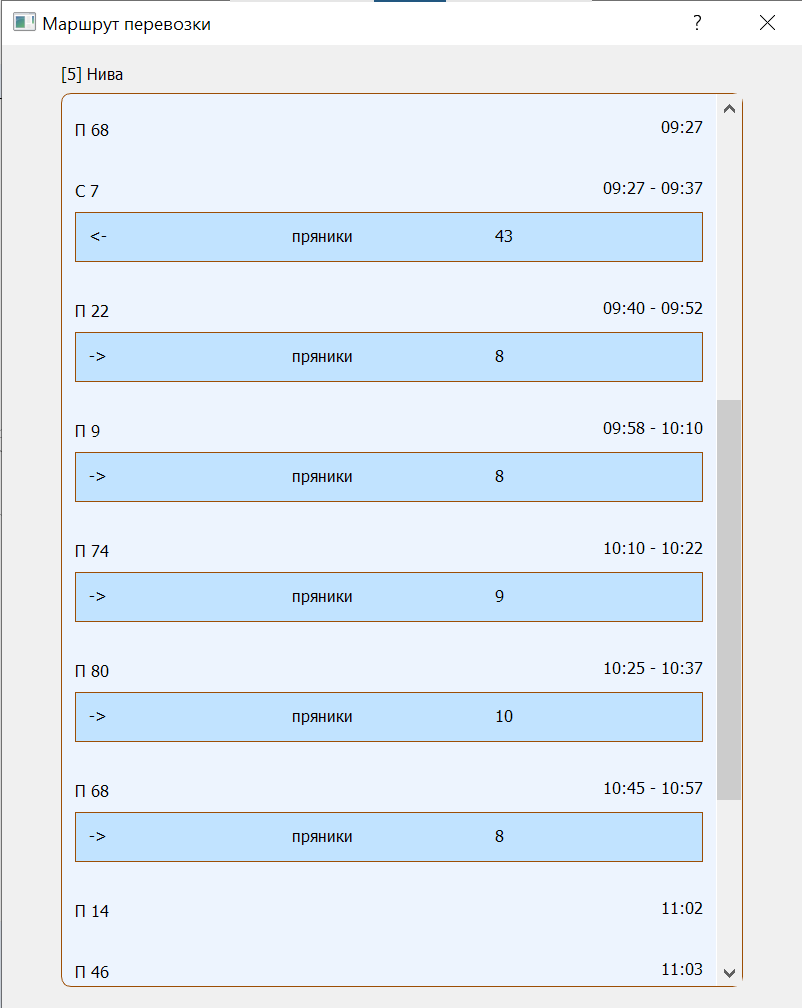
\includegraphics[scale=0.6, angle=0, page=1]{img/demo_route_2.png}}
		\caption{Пример 2. План маршрута}
		\label{demo:route2}
	\end{center}
\end{figure}

\begin{figure}[h!]
	\begin{center}
		{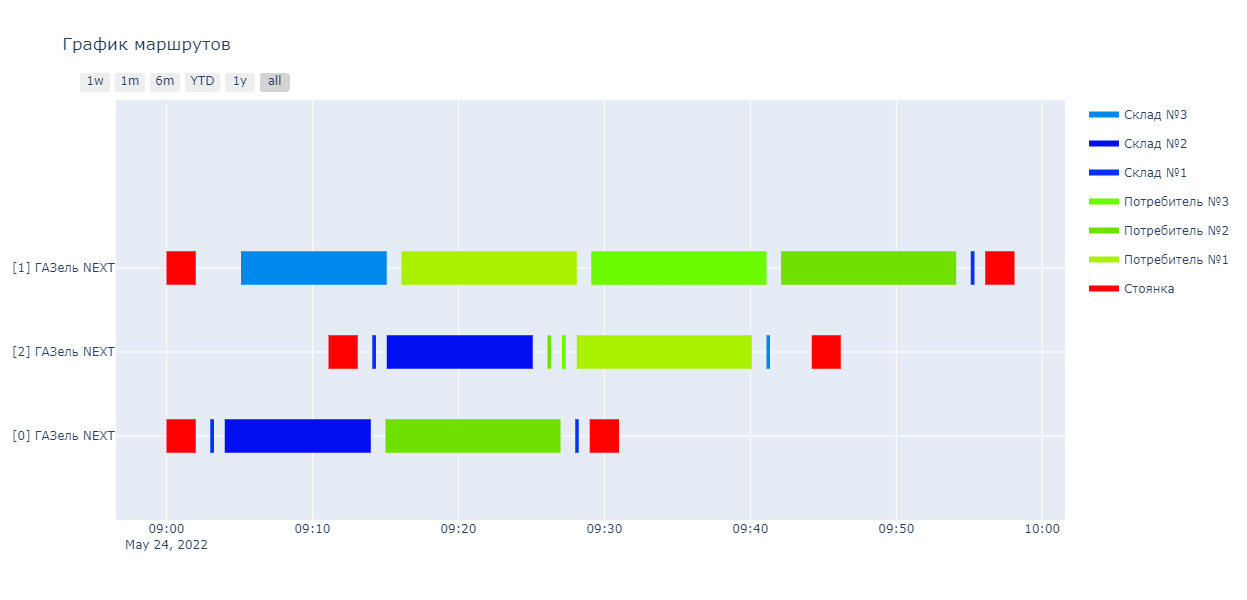
\includegraphics[scale=0.4, angle=0, page=1]{img/demo_schedule_1.png}}
		\caption{Пример 1. Временной график грузоперевозок}
		\label{demo:schedule1}
	\end{center}
\end{figure}

\begin{figure}[h!]
	\begin{center}
		{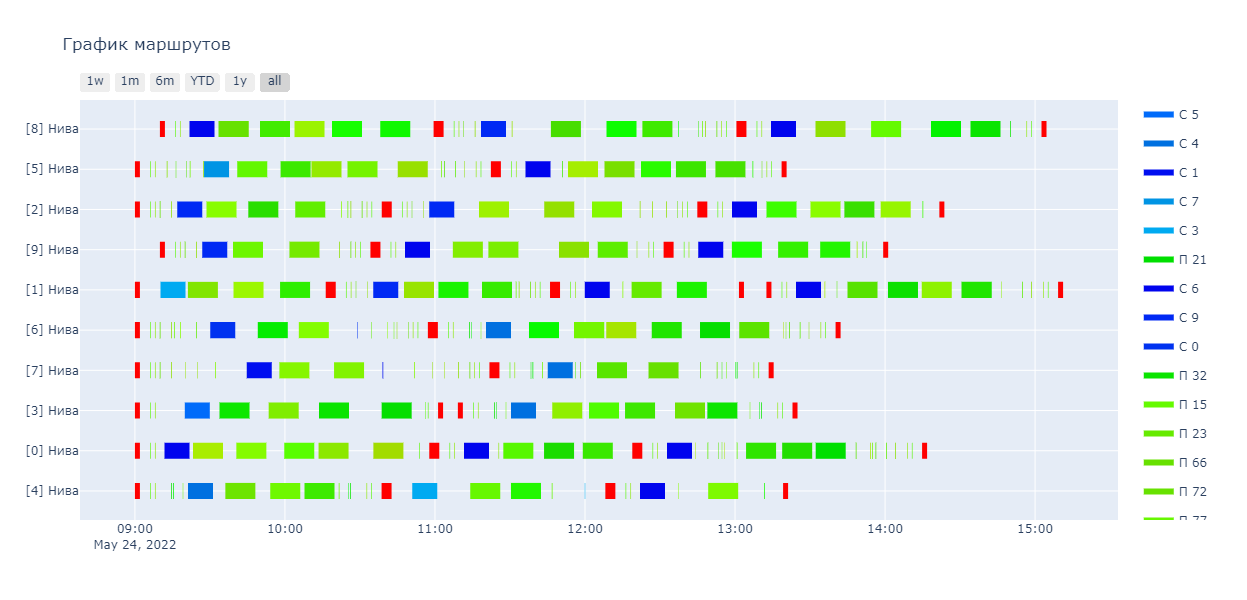
\includegraphics[scale=0.4, angle=0, page=1]{img/demo_schedule_2.png}}
		\caption{Пример 2. Временной график грузоперевозок}
		\label{demo:schedule2}
	\end{center}
\end{figure}

\newpage
\subsection{Тестирование программы}
Для поддержания работоспособности программы в процессе её разработки и было использовано автоматическое тестирование кода. Для этого была использован встроенный модуль unittest\cite{libs:unittest}. 

\pagebreak
Тестирование осуществлялось по методу чёрного ящика. В качестве входных данных выступали файлы с транспортными системами, подразумевающие различные сценарии оптимизации. В ходе одного теста проверялась корректность завершения работы методы, а также следующие выходные данные:

\begin{itemize}
	\item количество и стоимость маршрутов в плана (сравнивается с вручную вычисленным значением для данного теста);
	\item удовлетворение спроса потребителей;
	\item соблюдение ограничений запасов продукции и вместительности транспорта;
	\item целостность и замкнутость маршрутов.
\end{itemize}

В окончательной версии программы все тесты завершаются корректно.

\subsection*{Вывод}
Результатом технологической части стал выбор средств реализации программы, а также набора необходимых библиотек. В рамках созданного приложения был реализован ранее описанный метод оптимизации. Продемонстрирован и описан интерфейс, а также примеры работы программы. Разработанное программное обеспечение покрыто тестами.


\pagebreak